\documentclass[border=10pt]{standalone}
\usepackage{pgfplots}
\pgfplotsset{compat=1.18}
\begin{document}
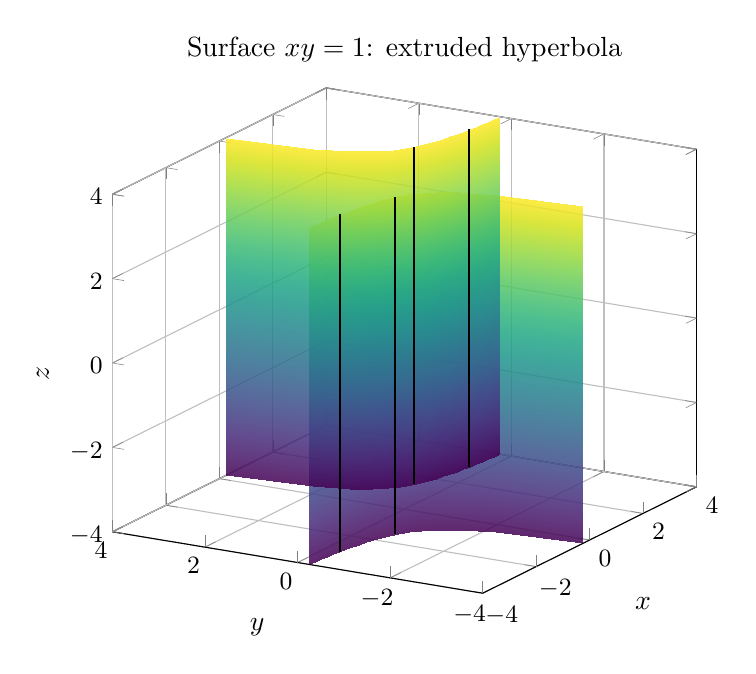
\begin{tikzpicture}
\begin{axis}[
    view={-60}{20},
    xlabel={$x$},
    ylabel={$y$},
    zlabel={$z$},
    xmin=-4, xmax=4,
    ymin=-4, ymax=4,
    zmin=-4, zmax=4,
    width=9cm, height=8cm,
    grid=major,
    tick label style={font=\small},
    title={Surface $xy=1$: extruded hyperbola},
]
\addplot3[
    surf, shader=interp, opacity=0.85,
    colormap/viridis,
    domain=-4:-0.25, samples=20,
    domain y=-4:4, samples y=8,
] ({x},{1/x},{y});
\addplot3[
    surf, shader=interp, opacity=0.85,
    colormap/viridis,
    domain=0.25:4, samples=20,
    domain y=-4:4, samples y=8,
] ({x},{1/x},{y});
\addplot3[black, thick, samples=2] coordinates {(3,1/3,-4) (3,1/3,4)};
\addplot3[black, thick, samples=2] coordinates {(1.5,2/3,-4) (1.5,2/3,4)};
\addplot3[black, thick, samples=2] coordinates {(-1.5,-2/3,-4) (-1.5,-2/3,4)};
\addplot3[black, thick, samples=2] coordinates {(-3,-1/3,-4) (-3,-1/3,4)};
\end{axis}
\end{tikzpicture}
\end{document}